%!TEX program = pdflatex
\documentclass{article}
\usepackage{graphicx}
\usepackage{pgffor}
\usepackage{geometry}
\usepackage{xcolor}
\usepackage{amsmath}
\usepackage[hidelinks]{hyperref}
\usepackage{url}

\title{$^{39}$Ar pdf parametrization test}
\date{\today}
\author{Automatically generated by \texttt{gipert/gerda-ar39-pdf}}

\def\chlista{%
  0, 1, 2, 3, 4, 5, 7, 9, 10, 11, 12, 13, 14, 15, 16%
}
\def\chlistb{%
  17, 18, 19, 20, 21, 22, 23, 24, 25, 26, 27, 28, 29, 30, 31%
}
\def\chlistc{%
  32, 33, 34, 35, 37, 38, 39, 40%
}

\begin{document}

\maketitle

Test plots of the estimated $^{39}$Ar pdf (in energy space) for each
\textsc{Gerda} Phase~II$^+$ detector and for various detector full
charge-collection depth (FCCD) and fully-dead layer fraction (DLF) hypotheses.

\begin{itemize}
  \item Interpolation strategy
    \begin{itemize}
      \item Monte Carlo simulations of $^{39}$Ar events in the \textsc{Gerda}
        PhaseII$^+$ setup are post-processed to fold in a linear model of the
        HPGes transition layer (n$^+$ contact, Fig.~\ref{fig1}). FCCD values
        are chosen in a 0.65:0.05:2.4\,mm grid, DLF values in a 0.0:0.1:10
        grid.
      \item To mitigate the effect of low statistics in the Monte Carlo
        histograms, an interpolation is made (interpolation in energy space) by
        drawing a cubic spline through 13\,keV bin contents. A 13\,keV bin
        width seems to perform well for all detectors. The MC histogram is
        normalized by the number of simulated \textsc{Geant4} primaries
        (technically this is not a pdf, it's a \emph{density}).
      \item The splines are saved on disk, resulting in a 4-dimensional lookup
        table (discretization) of the $^{39}$Ar pdf.
      \item the lookup table is loaded in memory for fast access by a separate
        program, which calculates the value of the pdf for each detector and in
        the full, continuous 3-dimensional parameter space of energy, FCCD and DLF:
        \begin{verbatim}
    double gerda::ar39_pdf(int ge_channel, double energy_kev,
                           double fccd_mm, double dlf);
        \end{verbatim}
        The interpolation is (tri)linear\footnote{\url{https://en.wikipedia.org/wiki/Trilinear_interpolation}}.
    \end{itemize}
  \item Reference dataset: full \textsc{Gerda} PhaseII$^+$ data. Energy
    resolution and run configurations are taken into account. The normalization
    factor resulting from a fit on data histograms can be easily converted into
    the measured $^{39}$Ar activity, given the dataset livetime.
\end{itemize}

\textcolor{red}{Red} pdfs
directly come from the internal lookup table, \textcolor{blue}{blue} pdfs are the
result of a trilinear interpolation.

\clearpage

\begin{figure}
  \centering
  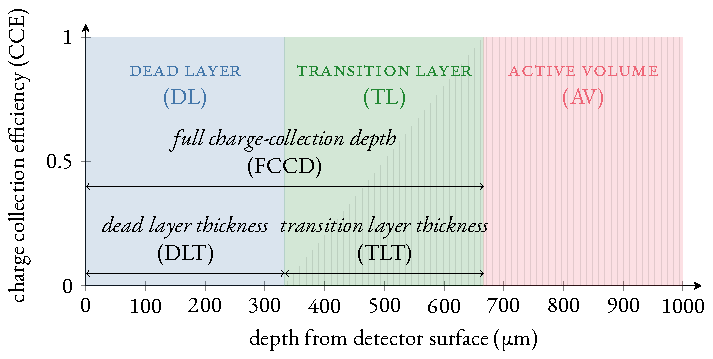
\includegraphics[width=0.8\textwidth]{tl-model.pdf}
  \caption{A linear model of the lithiated n$^+$ contact of an HPGe detector.}\label{fig1}
\end{figure}

\tableofcontents

\newgeometry{margin=2cm}

\foreach \fccd in {0.70mm,1.00mm,1.50mm,2.50mm}{%

  \section{DLF scan (FCCD = \fccd)}

  \begin{figure}[!ht]
    \centering
    \foreach \ch in \chlista{%
      \includegraphics[width=0.32\textwidth]{dlf/ch\ch-fccd\fccd.pdf}
    }
    \caption{DLF scan (FCCD = \fccd), see plot title for details}
  \end{figure}
  \begin{figure}[!ht]
    \centering
    \foreach \ch in \chlistb{%
      \includegraphics[width=0.32\textwidth]{dlf/ch\ch-fccd\fccd.pdf}
    }
    \caption{DLF scan (FCCD = \fccd), see plot title for details}
  \end{figure}
  \begin{figure}[!ht]
    \centering
    \foreach \ch in \chlistc{%
      \includegraphics[width=0.32\textwidth]{dlf/ch\ch-fccd\fccd.pdf}
    }
    \caption{DLF scan (FCCD = \fccd), see plot title for details}
  \end{figure}

  \clearpage
}

\foreach \dlf in {0.20,0.50,0.80}{%

  \section{FCCD scan (DLF = \dlf)}

  \begin{figure}[!ht]
    \centering
    \foreach \ch in \chlista{%
      \includegraphics[width=0.32\textwidth]{fccd/ch\ch-dlf\dlf.pdf}
    }
    \caption{FCCD scan (DLF = \dlf), see plot title for details}
  \end{figure}
  \begin{figure}[!ht]
    \centering
    \foreach \ch in \chlistb{%
      \includegraphics[width=0.32\textwidth]{fccd/ch\ch-dlf\dlf.pdf}
    }
    \caption{FCCD scan (DLF = \dlf), see plot title for details}
  \end{figure}
  \begin{figure}[!ht]
    \centering
    \foreach \ch in \chlistc{%
      \includegraphics[width=0.32\textwidth]{fccd/ch\ch-dlf\dlf.pdf}
    }
    \caption{FCCD scan (DLF = \dlf), see plot title for details}
  \end{figure}

  \clearpage
}

\foreach \dlf in {0.50}{%

  \section{FCCD fine scan (DLF = \dlf)}

  \begin{figure}[!ht]
    \centering
    \foreach \ch in \chlista{%
      \includegraphics[width=0.32\textwidth]{fccd/ch\ch-dlf\dlf-fine.pdf}
    }
    \caption{FCCD scan (DLF = \dlf), see plot title for details}
  \end{figure}
  \begin{figure}[!ht]
    \centering
    \foreach \ch in \chlistb{%
      \includegraphics[width=0.32\textwidth]{fccd/ch\ch-dlf\dlf-fine.pdf}
    }
    \caption{FCCD scan (DLF = \dlf), see plot title for details}
  \end{figure}
  \begin{figure}[!ht]
    \centering
    \foreach \ch in \chlistc{%
      \includegraphics[width=0.32\textwidth]{fccd/ch\ch-dlf\dlf-fine.pdf}
    }
    \caption{FCCD scan (DLF = \dlf), see plot title for details}
  \end{figure}

  \clearpage
}

\end{document}
